\chapter{High Frequency Trading}
\label{chapter:HFT}

\vspace{0.5cm} 

High frequency trading (HFT) strategies are based on buy and sell assets in
short periods of time gaining a small profit in every transaction despite the
transaction costs. The key is the amount of transactions that HFT algorithms are
capable to execute.  In 2012 more than 50\% of US market trades were HFT.  HFT
has motivated computer-driven strategies capable of processing large amount of
data in short periods of time. 


\section{High Frequency Trading Definition}

HFT is not a strategy but a technology that implements different trading
strategies. The aim of HFT is to benefit from market short-term pricing
inefficiencies~\cite{chlistalla2011}. HFT is characterised for the use of
high-speed and sophisticated quantitative and algorithmic computer applications
for modelling and executing orders efficiently. In order to make fast decisions,
HFT firms require speed access to trading servers and sometimes they are
physically near so they can minimise network latencies.

High frequency trades are short-term positions that commonly end the trading day
avoiding leaving opened positions to the next business day. HFT is frequently
associated to algorithm trading strategies, but the former is focused into
reduce the market impact of large institutional positions and the later refers
to trade execution strategies that are typically used by fund managers to buy or
sell large amounts of assets. The duration of the positions in HFT it is not
well-defined. Figure~\ref{fig:HFTtimes} shows a survey done to traders about the
holding time of a position opened. Most of them agreed that HFT refers to
positions between 1-second and 10-minutes. Overnight positions are avoided since
they are riskier and also have more expensive fees, HFT firms end the trading
day closing all opened positions.

\begin{figure}[!h]
  %\vspace{-0.8cm}
  \centering
  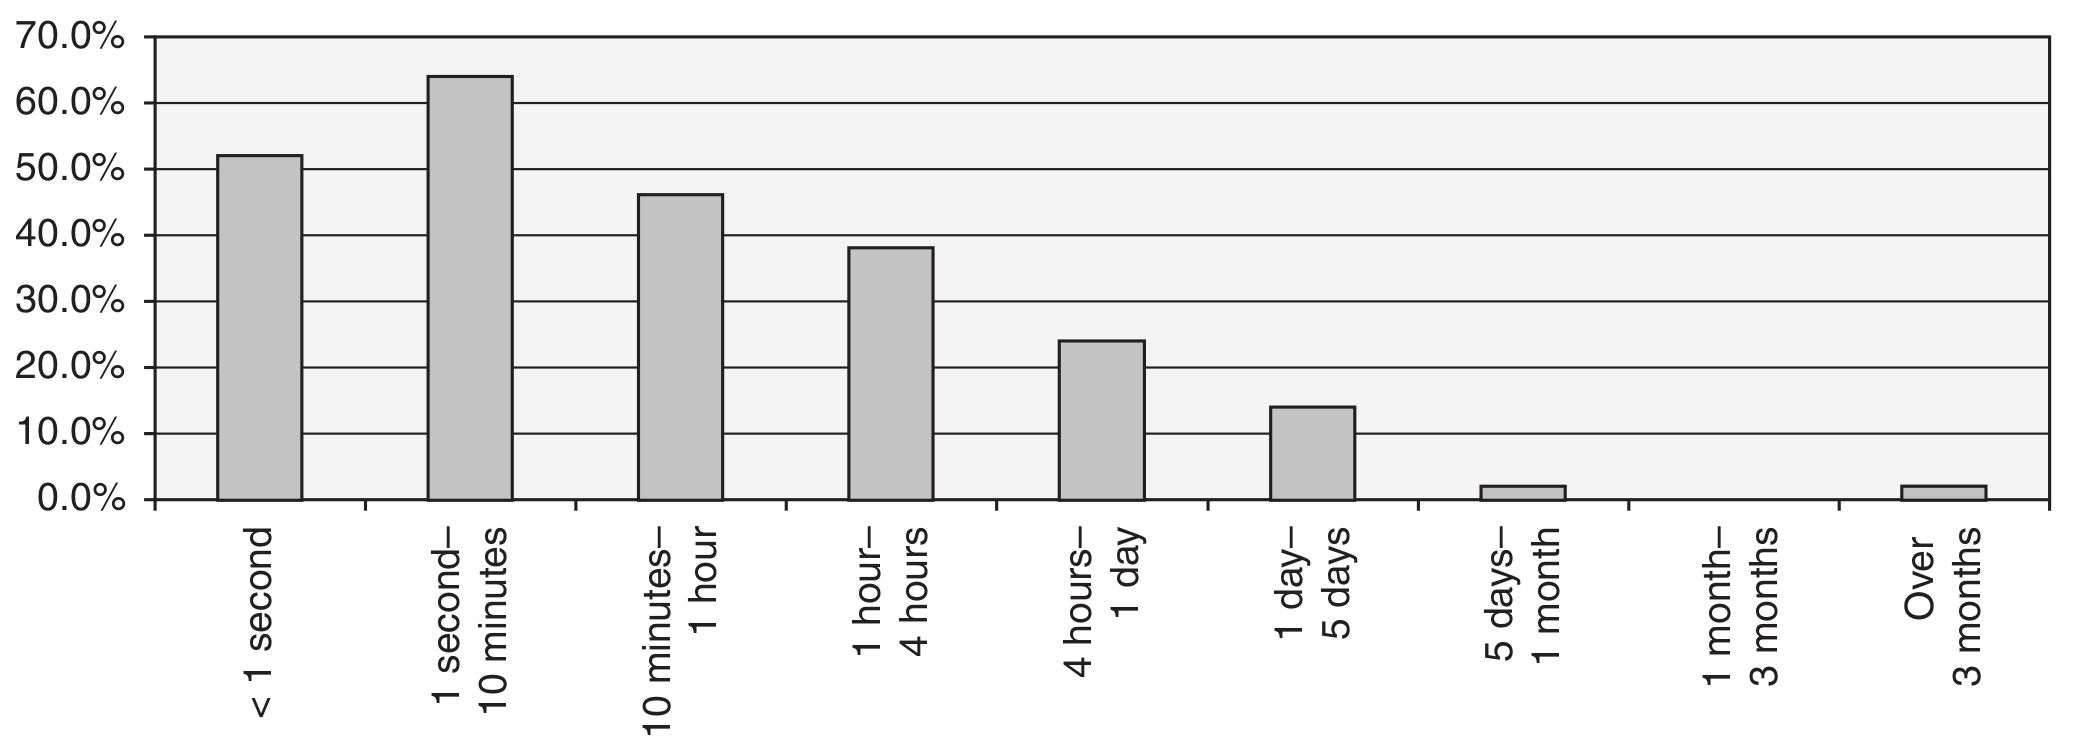
\includegraphics[width=\textwidth]{img/HFTtradestime}
  \caption{Holding time of an opened position of a high frequency trade.Source
  \cite{aldridge2009}.}
  \label{fig:HFTtimes}
\end{figure}
In 2014 HFT represented nearly 50\% of equity trades in the US and more than
20\% in Europe showing a consistent fall since 2009 which was its best year. US
market revenues have fallen dramatically.  Figure~\ref{fig:HFTmarket} on the
left shows HFT trades percentage of US and Europe equity shares. The right
figure shows how revenues in US stocks have fallen the last years.

\begin{figure}[!h]
  %\vspace{-0.8cm}
  \centering
  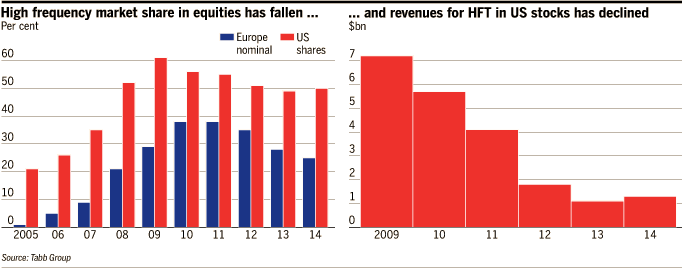
\includegraphics[width=\textwidth]{img/HFTmarket}
  \caption{Left figure shows HFT market share in the US and Europe. Right figure
  shows revenue in the US. Source: TABB Group.}
  \label{fig:HFTmarket}
\end{figure}
One of the reasons of this fall is that exchange markets have adapted, having
now faster, more transparent and efficient market structures than before.
This has been possible due to its investment in technology enhancing
reliability and stability of transactions. Even though this fall, HFT is still a major component of regulated markets and
will probably remain as a topic of interest for researchers in the near future.

On the other hand, HFT has been criticised on qualitative issues concerning
fairness and systemic risk. However, empirical research shows that HFT has lead to
beneficial impacts such as reducing spreads (difference between buyers and
sellers prices), increased liquidity, allowing more efficient price formation,
reduced transaction costs and lower market volatility. HFT makes the stock market more efficient and helps small investors who trade at random times over the day. 


\section{Financial Markets}

A financial market is any marketplace where buyers and sellers participate
trading different assets such as equities, bonds, currencies and derivatives
(future or options). One of the main objectives of financial markets is to set
prices for global trade.
A financial market has many components but the most commonly used are money
markets and capital markets. Money markets are used for short-term basis,
usually for assets up to one year, for greater periods capital markets are used.
Capital markets include the stock or equity market and the bond or debt market
and their movements are the most widely followed \cite{aldridge2009}.

\begin{figure}[!h]
  %\vspace{-0.8cm}
  \centering
  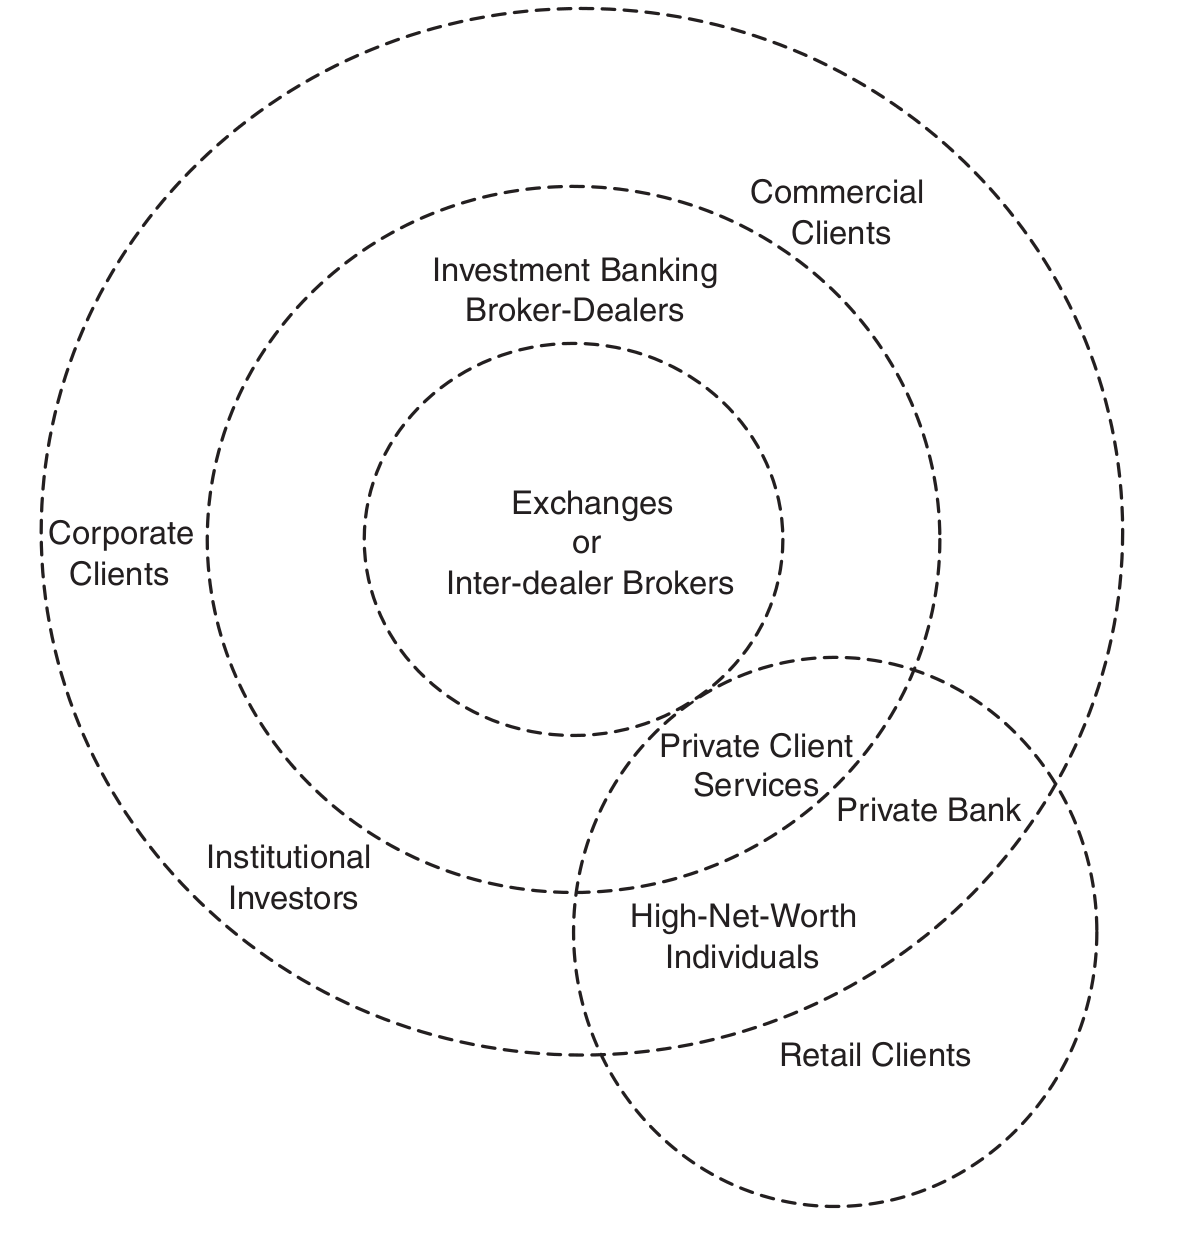
\includegraphics[width=0.7\textwidth]{img/capitalmarkets}
  \caption{Old structure of capital markets. Source \cite{aldridge2009}.}
  \label{fig:capitalmarket}
\end{figure}
Figure~\ref{fig:capitalmarket} shows the typical structure of capital markets
existed from the early 1929s through much of the 1990s where the broker-dealers
played the central and most profitable role.  At the core are the exchanges or
inter-dealer networks (foreign exchange trading). Exchanges are the centralised
marketplaces for transacting.  Broker-dealers perform two functions: trading for
their own accounts and transacting for their customers. Broker-dealers use
inter-dealer brokers to quickly find the best price for a particular asset among
the network of other broker-dealers. Occasionally, broker-dealers also deal
directly with other broker-dealers, particularly for less liquid instruments.
Broker-dealers clients are institutional investors, corporate clients,
commercial clients, and high-net-worth individuals \cite{aldridge2009}.

This centralised structure existed until computer technology allowed a better
communication structure. Today financial markets are more decentralised
providing more liquidity. Exchanges and inter-dealer brokers were replaced by
liquidity pools or Electronic Communication Networks (ECNs) which are able to
transmit order quickly matching buyers and sellers optimally. There are also
dark liquidity pools where trader identity and orders remain anonymous.

Figure~\ref{fig:capitalmarketnow} shows current structure of capital markets
including ECNs and dark pools. In this structure, ECNs, Exchanges, dark pools,
broker-dealers and retail brokerages can execute orders. However, there are some
institutional clients that have also become broke-dealers.

\begin{figure}[!h]
  %\vspace{-0.8cm}
  \centering
  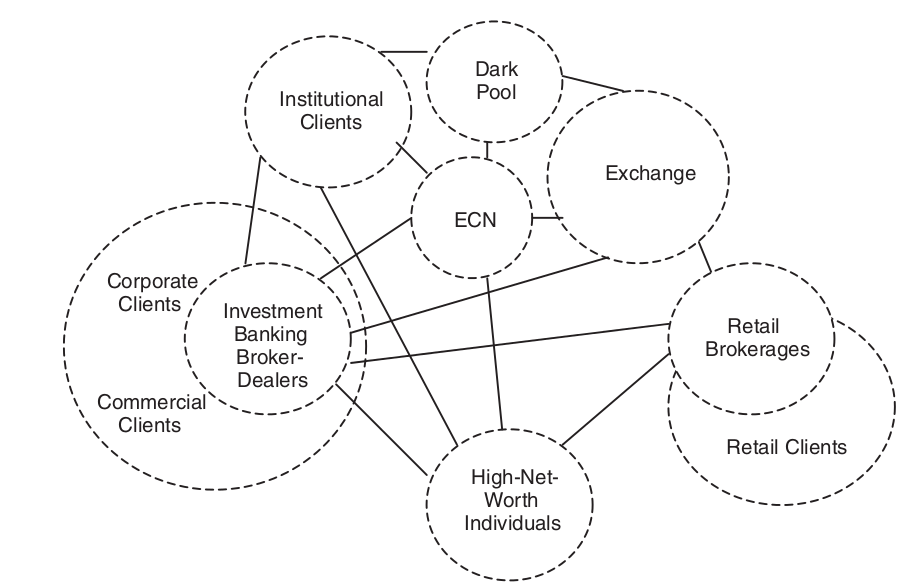
\includegraphics[width=0.8\textwidth]{img/capitalmarketsnow}
  \caption{Actual structure of capital markets. Source \cite{aldridge2009}.}
  \label{fig:capitalmarketnow}
\end{figure}


Equity market and foreign exchange market (Forex) are the most popular markets
for high frequency trading strategies \cite{genccay2001introduction}. In the
Equity market, stocks such as futures and options, exchange-traded funds (ETFs)
among others financial instruments can be traded. Additionally, in the Forex
market, interest rates denominated pair currencies such as EURUSD (Euro to UD
dollar) or USDJPY (US dollar to Japanese yen) are traded. Traders of this
market are diverse, some of them are high frequency traders, long-term
investors and corporations. The Forex market used to be centralised, only
commercial banks had exclusive access to inter-dealer networks. Today, Forex
market is decentralised and has become the biggest market in terms of volume of
trading. The main participants are international banks geographically dispersed
with continuous 24 hours operations excepting weekends.
Figure~\ref{fig:Forextimes} shows different market trading hours in GMT for
London, New York, Sydney and Tokyo.

\begin{figure}[!h]
  %\vspace{-0.8cm}
  \centering
  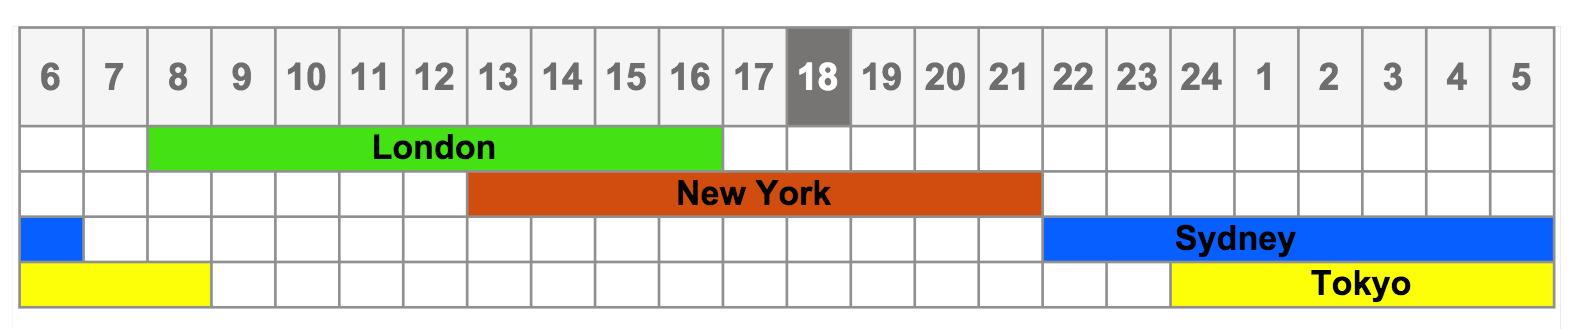
\includegraphics[width=0.8\textwidth]{img/forex-trading-hours.png}
  \caption{Forex market trading hours (GMT). Source \cite{dailyprice}.}
  \label{fig:Forextimes}
\end{figure}


There are three periods of overlaps between different trading times:

\begin{itemize}
\item New York and London from 13:00 GMT until 17:00 GMT
\item Tokyo and London from 8:00 GMT until 9:00 GMT
\item Sydney and Tokyo from 23:00 GMT to 7:00 GMT 
\end{itemize}

These overlap hours are very important since the highest volume of trades are
expected. Therefore, most HFT strategies are executed in these hours.

\section{Price formation process}

A trade consists at least of two orders: one to enter the market (buy order) and
exit the market (sell order). Traders have different types of order they can
execute:

\begin{description}
\item[Market order] allows to buy or sell an asset at the current best price
whatever the price is. The transaction price is determined by the market
considering previous executed orders and volume requested.
\item[Limit order] allow to specify the price you want to buy or sell an asset.
Depending on the market conditions, this type of orders could never been executed.
\item[Stop order] are suitable for investors who are unable to monitor their
investments for a period of time. Stop order allows to specify the price that a
position should be closed; this price is called stop price. When the stop price
is reached a market order is executed, this means that market price could not be
exactly the same specified in the stop order.
\end{description}

In terms of commissions, limit and stop order are more expensive than market orders and
there is no certainty of execution.

Moreover, all orders can specify other parameters such as: 

\begin{description}
\item[Fill or Kill] is an order that must be executed immediately or being
cancelled, no partial fulfillments are allowed. 
\item[Day] the order is only valid during the day.
\item[Good til canceled] a order is active until the investor decides to cancel
it or the trade is executed.
\end{description}

In order to determine the execution price, buyers and sellers orders are placed
in an order book which help to determine which order can be fulfilled.
Figure~\ref{fig:orderbook} illustrates how buyers and sellers are ordered. The
ask or offer price is the current lower price a seller is willing to accept for
a good. The bid price corresponds to the current highest price a buyer is
willing to pay for a good. Orders with the same price are prioritised by
arrival time and placed on top of the book.  The difference between current ask
and bid price is called spread and their average is called mid-price
\cite{bouchaud2002statistical}.

\begin{figure}[!h]
  %\vspace{-0.8cm}
  \centering
  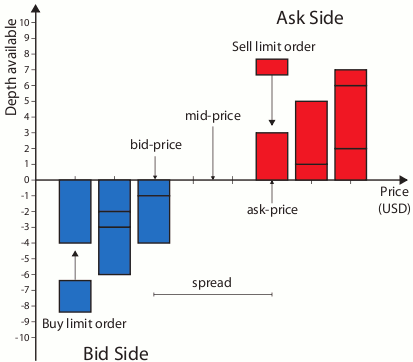
\includegraphics[width=0.5\textwidth]{img/orderbook}
  \caption{Order book. Buyers and sellers are ordered according to the bid or
ask price and the market determines the mid-price and transacted volume. Source
\cite{gould2013limit}.}
  \label{fig:orderbook}
\end{figure}
Today, order books are available and they are a popular source of study among
researchers. The mid-price and spread modelling are some of the
problems related with this area. 


\section{Efficient market hypothesis}

Efficient Market Hypothesis (EMH) was developed independently by  Paul
Samuelson and Eugene Fama in the 1960s.  EMH also known as the random walk
theory states that current stock prices fully reflect available information
related to its value and there is no way to earn excess profits
\cite{fama1970}. EMH requires that all the participants have rational
expectations, and investors reactions be random and follow a normal
distribution pattern. Thus, any one can be wrong about the market, but the
market is always right as a whole.  There are three common forms of EMH:
weak-form efficiency, semi-strong efficiency and strong-form efficiency.

The weak form claims that prices already reflect all past publicly available
information. Therefore, future prices cannot be predicted based on analysis of
historical data. This implies that future prices movements are determined
entirely by information not contained in the past prices and participants are
unable to systematically profit from market inefficiencies.  However, many
studies have shown a marked tendency for the stock markets to trend over time
periods. Various explanations for such large and apparently non-random price
movements have been promulgated. Even Fama has accepted price anomalies which
do not follow the weak-form efficiency hypothesis \cite{fama+french2008}.

The semi-strong form of the EMH claims that prices instantly change to reflect
new public (not private) information such that no excess return can be
obtained. 

The strong form of the EMH additionally claims that prices instantly reflect
even hidden, private or ``insider" information. 

EMH is related with two approaches to investment analysis: fundamental and
technical analysis. Fundamental analysts base their predictions of stock price
behaviour on fundamental factors such as internal information of a company, its
industry or the economy. Technical analysts, by contrast, consider that all
this financial information is already included in the prices and believe that
future stock prices can be predicted studying the historical market behaviour.
A market technician bases his predictions on historical patterns of prices of
volume changes.

Under the weak form of EMH, strategies based on technical analysis will not be
able to produce excess returns. However, the weak form accepts that some forms
of fundamental analysis may still provide excess return. Similarly, the
semi-strong form of EMH  neither technical or fundamental analysis can produce
excess return.

If the stock market efficiently digests all available information, there is
little justification for seeking excess returns gains from investing. However,
EMH doesn't lessen the importance of investing only change its philosophy. The
only way an investor can possibly obtain higher returns is by purchasing
riskier investments.

 Researches can determine now how efficient a financial market is, i.e how
efficiently information is processed.  

EMH is based on rational human behaviour and its validity has been criticised
by psychologists and behavioural economists who argue that the EMH is based on
counterfactual assumptions regarding human behaviour, that is, rationality.
Recent advances in evolutionary psychology and the cognitive neurosciences may
be able to reconcile the EMH with behavioural anomalies. On the other hand, if
the EMH is true, the market really walks randomly and therefore there shouldn't
be any difference between experienced and novice traders. Kim Man Lui proved
the contrary in a controlled experiment \cite{man2013}.

